\documentclass{article}
\title{Inferring generation-interval distributions from contact tracing data}
\author{Sang Woo Park, David Champredon and Jonathan Dushoff}

\usepackage{amsthm}
\usepackage{amsmath}
\usepackage{amssymb}
\usepackage{amsfonts}

\usepackage{hyperref}
\usepackage{natbib}
\usepackage{hyperref}
\bibliographystyle{chicago}
\date{\today}

\usepackage{xspace}
\newcommand*{\ie}{i.e.\@\xspace}

\usepackage{color}

\newcommand{\Rx}[1]{\ensuremath{{\mathcal R}_{#1}}} 
\newcommand{\Ro}{\Rx{0}}
\newcommand{\RR}{\ensuremath{{\mathcal R}}}
\newcommand{\tsub}[2]{#1_{{\textrm{\tiny #2}}}}

\newcommand{\comment}[3]{\textcolor{#1}{\textbf{[#2: }\textsl{#3}\textbf{]}}}
\newcommand{\jd}[1]{\comment{cyan}{JD}{#1}}
\newcommand{\swp}[1]{\comment{magenta}{SWP}{#1}}
\newcommand{\dc}[1]{\comment{blue}{DC}{#1}}
\newcommand{\hotcomment}[1]{\comment{red}{HOT}{#1}}

\begin{document}
\maketitle

\section{Introduction}

An epidemic can be characterized by its speed (exponential growth rate, $r$) and its strength (reproductive number, \RR).
Reproductive number, defined as the average number of secondary cases arising from a primary case, is of particular interest as it provides information about the final size of an epidemic [CITE].
However, directly measuring the reproductive number often requires knowledge of entire disease history and may not be feasible early in an epidemic [CITE].
Instead, the reproductive number can be \emph{indirectly} estimated from exponential grwoth rate, which can easily be estimated from incidence data [CITE].
These two quantities are linked by generation interval distributions \citep{wallinga2007generation}.

Generation interval is defined as the time between when a person becomes infected and when that person infects another person.
As each individual experiences different course of infection, \emph{individual} generation interval distribution varies among infectors [CITE sven].
Hence, the \emph{intrinsic} generation interval distribution, which provides link between $r$ and \RR, is a pooled distribution across all potential infections.

Due to individual variation in infection time, the observed generation interval distribution can change depending on when and how it is measured \citep{champredon2015intrinsic}. \jd{Other cites first. Maybe cite us later when talking about qualitative effects. We need to talk clearly also about censored intervals}
There are important distinctions to be made when estimating generation intervals: \emph{intrinsic} generation intervals are measured by evaluating the infectiousness of infected people,
%% without regard to actual infection events,
while \emph{observed} generation intervals refer to the time between actual infection events.
Observed generation intervals in turn can be \emph{aggregated} across time, measured \emph{forward} in time by looking at a cohort of individuals infected at the same time and asking when they infected others, or measured \emph{backward in time} by look at a cohort and asking when their infectors were infected.
When aggregated generation intervals are observed until a given time in an ongoing epidemic, we refer to these as \emph{censored} (or right-censored) intervals.

Early in the epidemic when depletion of susceptible is negligible, we expect the forward generation interval distribution to be similar to the intrinsic generation interval distribution.
As epidemic progresses, an infector is less likely to infect individuals later in time due to decrease in susceptibles and the distribution of forward generation intervals will be shorter than the intrinsic distribution.
\swp{While this statement is true, it relies on the assumption that forward generation will be measured after all infected individuals that are infected early have recovered. We should note (and maybe explore the idea) that forward GI may be affected by censoring.}

Conversely, when an epidemic is growing exponentially, as often occurs near the beginning of an outbreak, the number of newly infected individuals will be large relative to the number infected earlier on. 
A susceptible individual is thus relatively more likely to be infected by a newly infected individual, and the distribution of backward generation intervals will be shorter than the intrinsic distribution.
When epidemic is subsiding, most infections are caused by the remaining infectors, rather than new infectors, and the backward generation interval will be long.

In practice, generation intervals are measured by contact tracing throughout the course of an epidemic, usually aggregated to increase the amount of information available. 
\jd{I kind of feel like, if you go on forever, aggregated GIs approach intrinsic GIs. This obviously isn't true for a single epidemic (observed GIs are shorter overall). On the other hand, it obviously \emph{is} true if you add births and get to a stable equilibrium. So I guess the remaining question is, do we get convergence if we have stable cycles? What we think about this will affect how we write the rest of this P.} 
If observation goes on throughout the disease cycle, then (something about something).
On the other hand, if calculations are being done based on early-outbreak data, the available censored data is best thought of as a weighted average of backward generation-interval distributions; like them, the observed censored intervals will be shorter than intrinsic distributions.

\swp{Need a paragraph about spatial effect?}
\jd{Yes, we do!}

In this study, we explore the temporal and spatial variation in the observed generation interval obtained from contact tracing.
We show that using the observed generation interval distribution directly will always underestimate the reproductive number \swp{need to confirm this statement when we're done with the ms}. 
We provide a statistical framework of recovering the intrinsic generation interval distribution from the observed generation interval distribution.

\swp{Going to rename the sections... but I think I like the current order...}
\section{Measuring generation intervals - Theory}

Following [CITE], let $K(t)$ be the infection kernel. 
The reproduction number is defined as
$$
\RR = \int_0^\infty K(t).
$$
Then, the intrinsic generation interval distributions is defined as
$$
g(t) = \frac{K(t)}{\RR}.
$$
Intrinsic generation-interval distribution can be considered as an intrinsic characteristic of a single average infector in a fully susceptible population.

\swp{Insert renewal equation approach}

\subsection{Right-censored interval}

Assume that contact tracing is performed from the beginning of an epidemic to time $t$.
The number of infection occuring at time $s$ caused by infectors who were themselves infected at time $s-\tau$ is given by
\begin{equation}
i_{s-\tau}(s) = \RR i(s-\tau) g(\tau) S(s)
\end{equation}
Then, total number of secondary infections that are $\tau$ time steps apart and occur before time $t$:
\begin{equation}
\RR \int_\tau^t i(s-\tau) g(\tau) S(s) ds.
\end{equation}
Then, the censored interval at time $t$ is given by
\begin{equation}
c_t(\tau)= \frac{\RR \int_\tau^t i(s-\tau) g(\tau) S(s) ds}{\RR \int_0^t \int_x^t i(s-x) g(x) S(s) ds dx}.
\end{equation}
We note that the expression in the denominater is equivalent to cumulative incidence at time $t$.
The intuition behind this is that we are normalizing acrosss all incidence before time $t$.
Then, we have
\begin{equation}
c_t(\tau) = \frac{\RR \int_\tau^t i(s-\tau) g(\tau) S(s) ds}{\int_0^t i(s) ds}.
\end{equation}
For convenience, we ignore normalizing constants and write
\begin{equation}\label{eq:obsg}
c_t(\tau) \propto g(\tau) \int_{0}^t i(s-\tau) S(s) ds.
\end{equation}

For a single epidemic, the observed mean generation interval through contact tracing will always be shorter than intrinsic mean generation interval (Figure~\ref{fig:censor}).
There are two reasons for this phenomenon.
First, as contact tracing is performed up to time $t$, any infection events that occur after time $t$ are not observed.
Any individuals that are infected before time $t$ can only complete infection events that are shorter than time $t$ and the distribution of all infection events that occur before time $t$ will be concentrated on shorter intervals.
In particular, when an epidemic is growing exponentially ($i(t) \propto \exp(rt)$), the censored generation interval distribution is equivalent to the inverse exponentially weighted intrisnc generation interval distribution:
\begin{equation}
\tsub{c}{exp}(\tau) \propto g(\tau) \exp(-r\tau),
\end{equation}
Second, number of susceptibles decrease over the course of an epidemic and any infector is less likely to infect susceptible individuals through long generation intervals than it would have in a fully susceptible population \citep{champredon2015intrinsic}.
As a result, even if contact tracing is performed through an entire epidemic, mean generation interval will be underestimated.

\begin{figure}
% 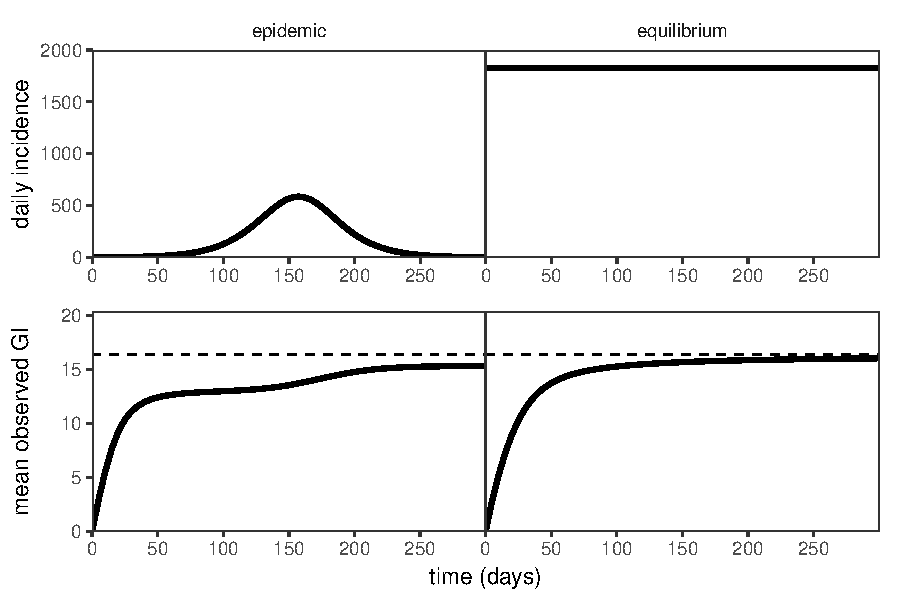
\includegraphics[width=\textwidth]{../contact_trace/temporal_effect.pdf}
\caption{Fill this out and re-do simulation with realistic Ebola parameters for consistency.}
\label{fig:censor}
\end{figure}

When an epidemic is in an equilibrium state (i.e., incidence $i(t)$ and the number of susceptibles $S(t)$ is constant over time), the observed generation interval distribution is equivalent to the intrinsic generation interval distribution. \swp{TODO: make a figure}
On the other hand, when an epidemic is in a cycle, we get ???

\subsection{Local depletion of susceptibles}

\swp{cite trapman somewhere}
The intrinsic generation-interval distribution is often defined as the distribution of times at which secondary infections occur [CITE].
This definition implicitly assumes that all infectious contacts made give rise to infection. 
Given limited contact network, depletion of susceptibles occur locally and the same person can be contacted multiple times.
Infectious contacts give rise to an infection only when the susceptible individual is contacted for the first time.
Therefore, the intrinsic generation-interval distribution is the distribution of times at which infectious contacts are made.

The \emph{effective} generation-interval distribution -- the distribution of times at which secondary infections occur -- depends on the probability that a susceptible individual has not been contacted yet and the intrinsic generation-interval distribution.
Given a constant per pair contact rate, $\beta(t)$, the effective generation-interval distribution is given by \swp{Need to double check this and/or make it more general.}
\begin{equation}
\tsub{g}{eff}(\tau) \propto g(\tau) \exp\left(-\int_0^{\tau} \beta(t) dt\right).
\end{equation}
Typically, when homogeneous contact and constant contact rates are assumed,
the per pair contact rate is sufficiently small ($\RR/N$ where $N$ is the population size) that the effect of local depletion of susceptibles is negligible.

The difference between effective and intrinsic generation-interval distribution can be best demonstrated by using a tree network: a single infector connected to small number of susceptible individuals (Figure ???).




\section{Statistical approach to estimating generation-interval distribution}

The observed generation-interval distribution is a weighted intrinsic generation-interval distribution (equation~\ref{eq:obsg}),
Then, the intrinsic generation interval can be recovered by taking the inverse weights:
\begin{equation}
g(\tau) \propto g_t(\tau) \frac{1}{\int_{0}^t i(s-\tau) S(s) ds}
\end{equation}
However, this method requires a knowledge of susceptible dynamics and may not be feasible in practice.

During exponential growth period, we can write $i(\tau) \propto \exp(r t)$, where $r$ is the exponential growth rate.
Assuming that $S(t) \approx 1$, the observed generation-interval distribution during growth period can be written as follows:
\begin{equation}
\tsub{g}{exp}(\tau) \propto g(\tau) \exp(-r\tau),
\end{equation}
Taking the inverse weight, we obtain the following expression for the intrinsic generation-interval distribution:
\begin{equation}
g(\tau) \propto \tsub{g}{exp}(\tau) \exp(r\tau)
\end{equation}
and the reproductive number:
\begin{equation}
\RR = \int_0^\infty \tsub{g}{exp}(\tau) \exp(r\tau) d\tau.
\end{equation}
Therefore, applying the Lotka-Euler equation using the observed generation interval via contact tracing results in underestimation of reproductive number:
\begin{equation}
\int_0^\infty \tsub{g}{exp}(\tau) \exp(r\tau) d\tau > \left(\int_0^\infty \tsub{g}{exp}(\tau) \exp(-r\tau) d\tau\right)^{-1}
\end{equation}
This method provides a non-parametric approach for inferring the intrinsic generation-interval distribution and the reproductive number from contact tracing data.

\swp{Need to rewrite this section. It's merely a place holder for now:}
While the non-parametric method is simple, it does not use all available information from contact tracing data.
In particular, it does not take into account who infected whom.
Assuming a poisson process, we can obtain a likelihood for observing infections:
\begin{equation}
\RR^{n_e} \cdot \prod g(\tau_e) \cdot \exp \left(- \RR \int_0^{c - t_{\tiny\textrm{inf}}} g(s) ds \right)
\end{equation}
This method requires us to make an assumption about the generation-interval distributions... See example...




\section{Methods}



\bibliography{network}
\end{document}
